%%% Local Variables:
%%% mode: latex
%%% TeX-master: t
%%% End:
\documentclass[a4paper, 11pt]{exam}
\usepackage[T1]{fontenc}
\usepackage{titling}
\usepackage{url}
\usepackage{amsmath,amsthm,amssymb}
\usepackage{graphicx}
\usepackage{graphics}
\usepackage{listings}
\usepackage[dvipsnames]{xcolor}
\usepackage{tabularx}
\usepackage{ragged2e}
\usepackage{courier}
\usepackage{textcomp}
\usepackage{circuitikz}
\usepackage{tikz}
\usetikzlibrary{shapes,arrows}
\usepackage{enumitem }
\usepackage{karnaugh-map}
\usepackage{bytefield}
\usepackage{mathrsfs}
\usepackage{cancel}
\usepackage[linesnumbered,ruled,vlined]{algorithm2e}
\usepackage{hyperref}

\newcommand{\invlaplace}[1]{%
\mathscr{L}^{-1}\left\{#1\right\}
}
\newcommand{\laplace}[1]{%
\mathscr{L}\left\{#1\right\}
}
\newcommand{\fourier}[1]{%
\mathscr{F}\left\{#1\right\}
}

\newcommand{\ztransform}[1]{%
\mathscr{Z}\left\{#1\right\}
}

\newcommand{\subtitle}[1]{%
  \posttitle{%
    \par\end{center}
    \begin{center}\large#1\end{center}
    }%
}

\usepackage{environ}

\NewEnviron{eqnsection}[2]{%
  \newcommand{\myvspace}{#1}%
  \vspace{\myvspace}%
  \begin{align*}
  \intertext{#2}
  \BODY
  \end{align*}%
  \vspace{\myvspace}%
}


\newcommand{\uparrowat}[1]{\underset{\uparrow}{#1}}


\newlist{myenumerate}{enumerate}{2}
\setlist[myenumerate,1]{label=\roman*)}
\setlist[myenumerate,2]{label=\alph*)}



\newcommand\tab[1][1cm]{\hspace*{#1}}

\renewcommand{\labelenumi}{\alph{enumi})}

\title{\textbf{Discrete Systems}}
\subtitle{ECE 6530: Digital Signal Processing}
\author{ Miguel Gomez U1318856\\} 


\begin{document}
\maketitle
\section{Sequence representation}
\label{sec:representations}
\begin{enumerate}
\item Functional
\item Tabular
\item Sequence
\end{enumerate}
\begin{center}
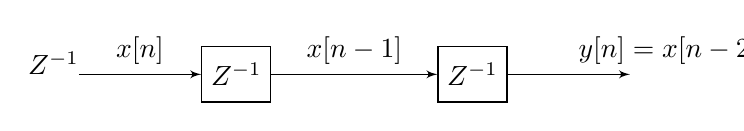
\begin{tikzpicture}[>=latex']
    \tikzstyle{block} = [draw, shape=rectangle, minimum height=2em, minimum width=2em];
    \tikzstyle{sum} = [draw, shape=circle, node distance=3.5cm];
    \tikzstyle{input} = [coordinate];
    \tikzstyle{output} = [coordinate];
    \tikzstyle{time_delay} = \node [block, node distance=3cm] (name) {$Z^{-1}$};
    
    % Nodes
    \node [input, name=input] {};
    \node [block, right of=input, node distance=2cm] (block1) {$Z^{-1}$};
    \node [block, right of=block1, node distance=3cm] (block2) {$Z^{-1}$};
    \node [output, right of=block2, node distance=2cm] (output) {};

    % Paths
    \draw [->] (input) -- node [name=x,above] {$x[n]$} (block1);
    \draw [->] (block1) -- node [name=mid,above] {$x[n-1]$} (block2);
    \draw [->] (block2) -- node [anchor=south west][name=y] {$y[n] = x[n-2]$} (output);
\end{tikzpicture}
\end{center}
\end{document}